\section{Einführung}

Das Restgasspektrum wurde wie in der Einführung beschrieben aufgenommen. Es wurde allerdings nicht der ganze Messbereich erfasst, sondern nur der Bereich von 1-50\;u, da fast alle erwarteten Elemente sich in diesem Spektrum befinden.\\
Wie in Abbildung \ref{fig:untergrund_1} zu sehen ist, wurden Peaks bei m = \{1, 2, 16, 17, 18, 19, 28, 32, 44\} u gemessen. Die kleineren Peaks um 18\;u entsprechen dabei dem Cracking-Pattern von Wasser, hierbei handelt es sich also um Bruchmoleküle, die aus dissoziiertem
H$_2$O entstanden.\\
Bei den restlichen Peaks der schwereren Elemente handelt es sich um molekularen Stickstoff (N$_2$, m = 28\;u), molekularen Sauerstoff (O$_2$, m = 32\;u) und Kohlenstoffdioxid (CO$_2$, m = 44\;u).\\

\begin{figure}[h]
	\centering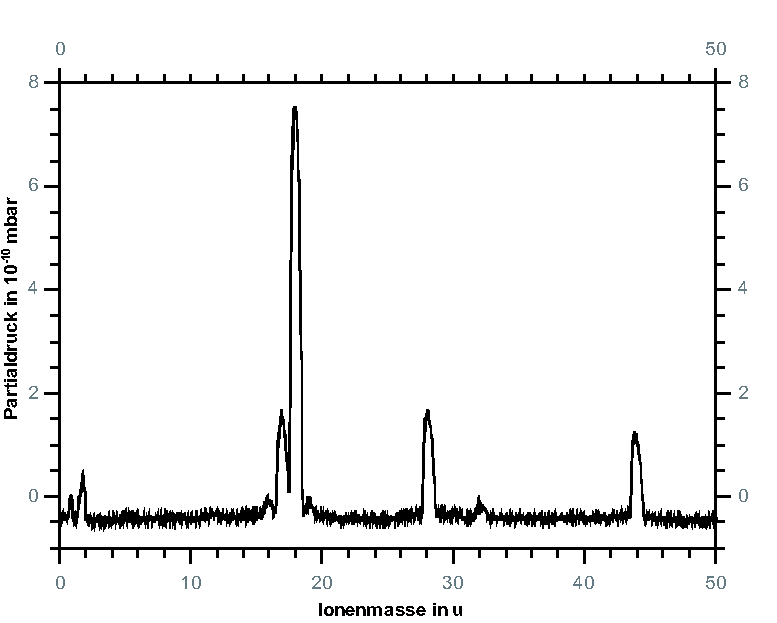
\includegraphics[width=0.8\textwidth]{fig/untergrund_1}
	\caption{Untergrundspektrum des Restgases}
	\label{fig:untergrund_1}
\end{figure}

Zur Bestimmung des Auflösungsvermögens wird, wie in der Vorbereitung beschrieben, die z\%-Linienbreite Definition verwendet, wobei z=20 gewählt wurde.\\
Dafür wurde noch einmal mit höherer Abtastrate die Massenbereiche 1-5\;u und 25-30\;u gemessen.\\
Wie erwartet steigt das Auflösungsvermögen mit steigendem m. Dies liegt daran, dass die Linienbreite $\Delta m$ bei unterschiedlichen Massenzahlen hinreichend konstant ist, zumindest immer <1, wobei die Massenzahl monoton steigt.\\
\begin{figure}[h]
	\centering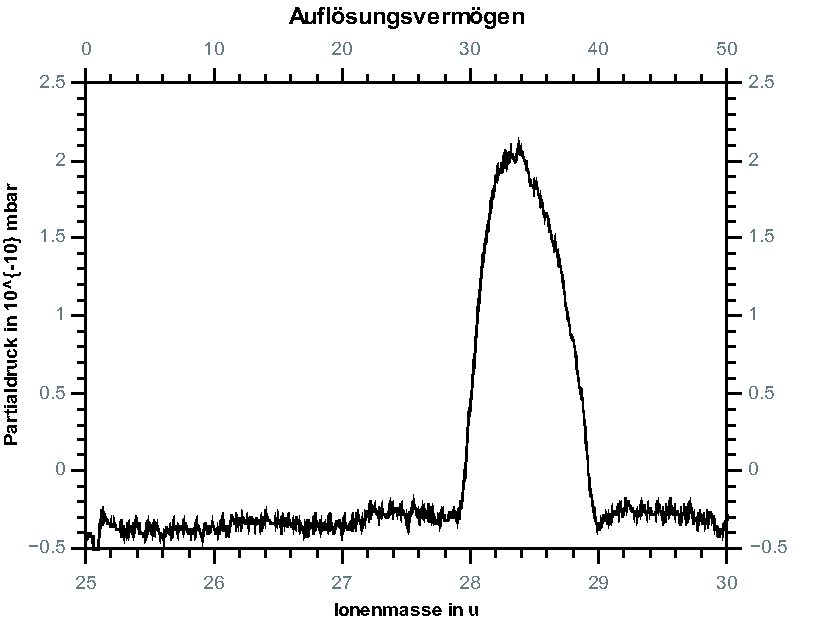
\includegraphics[width=0.8\textwidth]{fig/aufloesung}
	\caption{Genaue Aufnahme im Bereich von 25-30 u}
	\label{fig:aufloesung}
\end{figure}
Die Werte für m = 28\;u wurden Abb. \ref{fig:aufloesung} entnommen, der Rest dem großen Untergrundspektrum.
\begin{tabular}{ccc}
	\toprule
	$m$ in u&$\Delta m$ in u&R\\
	\midrule
	2&0.56&3.57\\
	18&0.94&19.15\\
	28&0.89&31.46\\
	\bottomrule
\end{tabular}

\section{Auftrittsenergie von Argon}
\label{sec:argon}

Um die Auftrittsenergie von Argon zu bestimmen, wurde die Vakuumkammer bis zu einem Druck von $4\cdot 10^{-6}$\;mbar mit Argon befüllt.
Anschließend wurde das Massenspektrometer auf m = 40\;u und m = 20\;u zur Detektierung von respektive Ar$^{+}$ und Ar$^{++}$-Ionen eingestellt.\\
Die Beschleunigungsspannung und damit Energie der stoßenden Elektronen konnte über einen Drehregler direkt gesteuert werden, wobei darauf geachtet unter einer Energie von 100\;eV zu bleiben.
Auf diese Weise wurde der Partialdruck der Argonionen in Abhängigkeit der Elektronenenergie gemessen.

\begin{figure}[h]
	\centering
	\subfigure[]{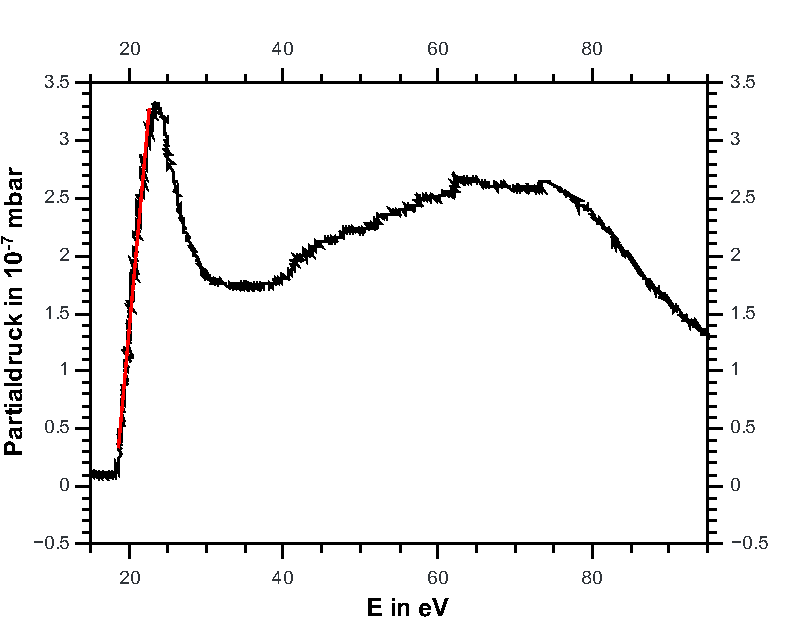
\includegraphics[width=0.49\textwidth]{fig/argon+}}
	\subfigure[]{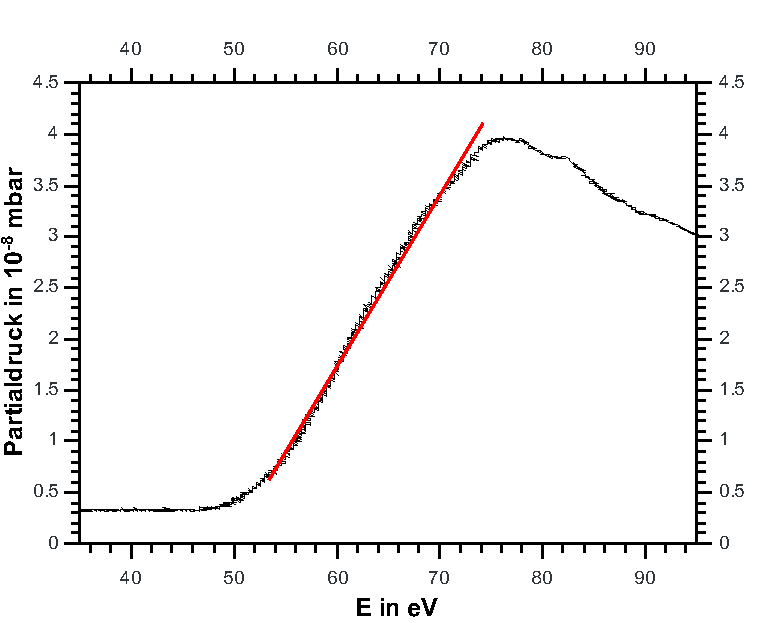
\includegraphics[width=0.49\textwidth]{fig/argon++}}
	\caption{\textbf{a)} Partialdruck in Abhängigkeit der Elektronenenergie bei m = 40\;u (Ar$^+$), \textbf{b)} Partialdruck in Abhängigkeit der Elektronenenergie bei m = 20\;u (Ar$^{++}$)}
	\label{fig:plot_argon}
\end{figure}

Wie erwartet nimmt der Partialdruck erst linear zu wodurch man mit einer Regression in diesem Bereich die Auftrittsenergie bestimmen kann.
\begin{equation}
	p(E) = m\cdot E + c
\end{equation}
Der Schnittpunkt dieser Geraden mit der x-Achse entspricht dann der Auftrittsenergie
\begin{equation}
	E_a = -\frac{c}{m}
\end{equation}

Die Regression im linearen Bereich wurde mit Qtiplot durchgeführt, welches auch direkt den statistischen Fehler liefert. Die lineare Regression ergibt folgende Geraden:
\begin{align}
	\textrm{p}_{Ar+}(E) &= \left((0,7356\pm 0,0125)\cdot\frac{E}{eV} - (13,350\pm 0,2533)\right)10^{-7}\textrm{mbar}\\
	\textrm{p}_{Ar++}(E) &= \left((0,1673\pm 0,0005)\cdot\frac{E}{eV} - (8,3097\pm 0,0334\right)10^{-8}\textrm{mbar}
\end{align}
Mittels Gaußscher Fehlerfortpflanzung (Gl. \ref{eq:gauss}) ergibt sich für die Auftrittsenergien:
\begin{align}
	E_{a,Ar+} &= \SI{18,15\pm 0,46}{\electronvolt}\\
	E_{a,Ar++} &= \SI{49,67\pm 0,25}{\electronvolt}
\end{align}
Vergleicht man die gemessenen Werte mit den Literaturwerten (E$_{a,Ar+}$ = 15,76\;eV, E$_{a,Ar++}$ = 43,39\;eV, \cite{Litmap}) so ergibt sich eine Abweichung von 15,2\;\% für einfach, bzw 14,5\;\% für zweifach ionisiertes Argon.\\
In beiden Fällen liegt der Literaturwert außerhalb der Fehlergrenzen und die Werte sind deutlich höher als erwartet. Dies könnte an nicht beachteten systematische Fehlern liegen, oder an der Durchführung des Versuchs, da die Beschleunigungsspannung per Hand geregelt werden musste und somit nicht wirklich linear anstieg.\\
\begin{equation}
	\Delta E_a = \sqrt(\left(\frac{\partial E_a}{\partial c}\cdot\Delta c\right)^2 + \left(\frac{\partial E_a}{\partial m}\cdot\Delta m\right)^2)
	\label{eq:gauss}
\end{equation}

\section{Dissoziationsenergie von Stickstoff}

Wie in der Vorbereitung beschrieben (\ref{sec:v3}) müssen als Erstes die Auftrittsenergien von N$^+$ und N$_2^+$ bestimmt werden. Dabei wird analog zum vorherigen Versuch verfahren (\ref{sec:argon}).\\
\begin{figure}[h]
	\centering
	\subfigure[]{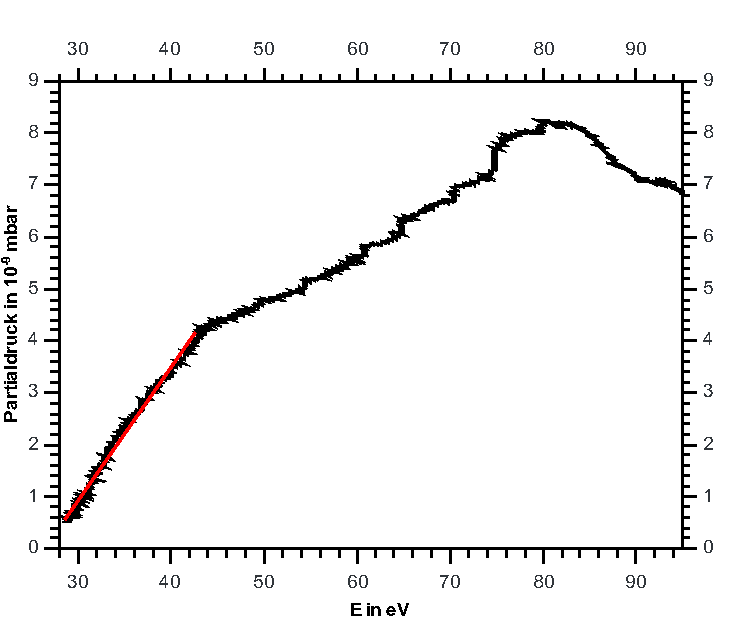
\includegraphics[width=0.49\textwidth]{fig/n+}}
	\subfigure[]{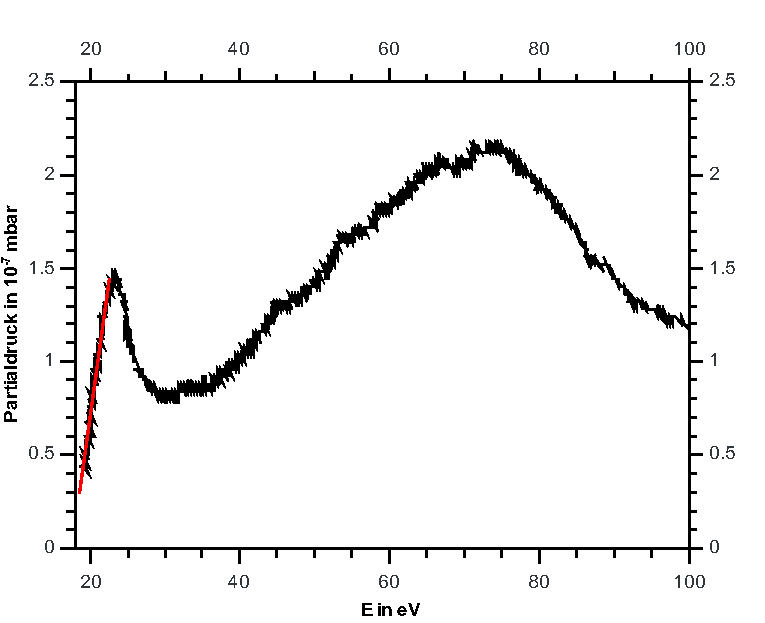
\includegraphics[width=0.49\textwidth]{fig/n2+}}
	\caption{\textbf{a)} Partialdruck in Abhängigkeit der Elektronenenergie bei m = 14\;u (N$^+$), \textbf{b)} Partialdruck in Abhängigkeit der Elektronenenergie bei m = 28\;u (N$_2^{++}$)}
	\label{fig:plot_stickstoff}
\end{figure}
Es ergeben sich die folgenden Regressionsgeraden:
\begin{align}
\textrm{p}_{N+}(E) &= \left((0,2571\pm 0,0011)\cdot\frac{E}{eV} - (6,7936\pm 0,0383)\right)10^{-9}\textrm{mbar}\\
\textrm{p}_{N++}(E) &= \left((0,2873\pm 0,0056)\cdot\frac{E}{eV} - (5,0472\pm 0,1152\right)10^{-7}\textrm{mbar}
\end{align}
Mittels Gaußscher Fehlerfortpflanzung (Gl. \ref{eq:gauss}) lässt sich die Auftrittsenergie mit Unsicherheit bestimmen:
\begin{align}
E_{a,N+} &= (26,42\pm 0,19)\;eV\\
E_{a,N_2^+} &= (17,57\pm 0,53)\;eV
\end{align}
Mit Kenntnis der Ionisationsenergie von Stickstoff (E$_\textrm{I}$ = 14,5\;eV) können nun die Dissoziationsenergien bestimmt werden:
\begin{align}
	E_\textrm{D}(N_2) &= E_a(N^+) - E_a(N_2^+) = (11,92\pm 0,56)\;eV\\
	E_\textrm{D}(N_2^+) &= E_a(N^+) - E_\textrm{I} = (8,85\pm 0,19)\;eV
\end{align}
Vergleicht man die gemessenen Werte mit den Literaturwerte (E$_\textrm{D}$(N$_2^+$) = 8,713\;eV, E$_\textrm{D}$(N$_2$) = 9,759\;eV, \cite{kobra}) so
ergibt sich eine Abweichung von 22,1\% für neutrales, bzw 1,6\% für einfach ionisierten molekularen Stickstoff.\\
Das Ergebnis für einfach ionisierten Stickstoff ist also sehr gut, obwohl der Messwert für neutralen Stickstoff relativ weit abweicht. Dies kann an einem nicht beachteten systematischen Fehler liegen, der bei beiden Messungen in die gleiche Richtung verfälscht. Dies würde erklären, warum die Differenz zweier Messwerte ein gutes Ergebnis liefert, wenn aber ein Literaturwert abgezogen wird, eine recht große Abweichung nach oben zu sehen ist.\\

\section{Versuch 4: Quantitative Analyse der Raumluft}

In diesem Versuch wird die Zusammensetzung der Luft bestimmt. Dazu wird Luft bis zu einem Druck von $p=\SI{3,7e-6}{\milli\bar}$ in den Rezipienten geleitet. Dann werden zwei Massenspektren aufgenommen. Aus der Höhe der Peaks lässt sich der Partialdruck des entsprechenden Gases bestimmen. Es gilt nämlich
\begin{equation}
 h = sp,
\end{equation}
mit der Peakhöhe $h$, der Sensitivität $s$ und dem Partialdruck des Gases $p$. Insgesamt lässt sich so der Anteil der verschiedenen Gase an der Luft bestimmen.

Zunächst wird ein Spektrum bei einem Messbereich von $\SI{e-7}{\milli\bar}$ aufgenommen (s. Abb. \ref{fig:v41}), um die Linie bei $\SI{28}{\amu}$, die deutlich höher als die anderen Linien ist, zu vermessen. Dann wird ein Spektrum bei $\SI{e-8}{\milli\bar}$ aufgenommen (s. Abb. \ref{fig:v42}), um auch die Höhe der niedrigeren Linien zu bestimmen.
Bei den Linien, die in beiden Spektren zu sehen sind, wird für die Auswertung der Mittelwert verwendet.

\begin{figure}[tb]
	\centering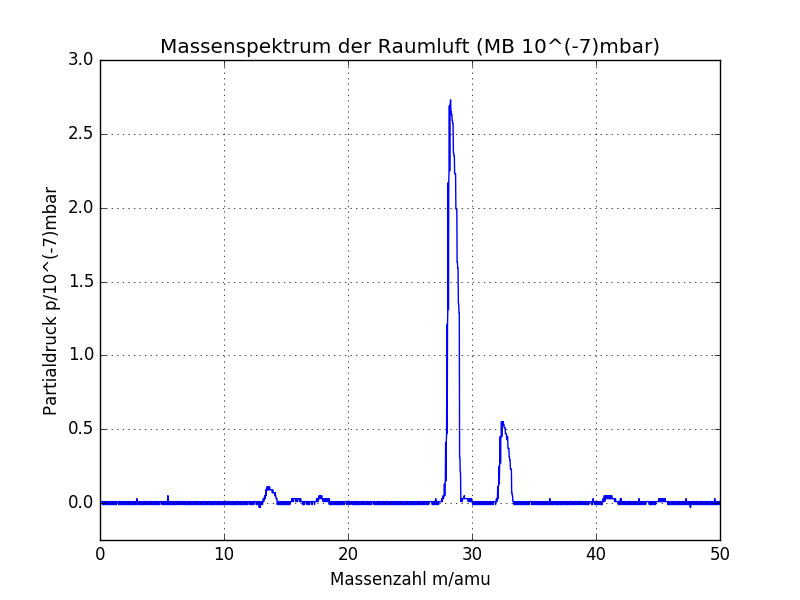
\includegraphics[width=0.9\textwidth]{fig/a4_1.png}
	\caption{Massenspektrum der Luft (Messbereich: $\SI{e-7}{\milli\bar}$)}
	\label{fig:v41}
\end{figure}

\begin{figure}[tb]
	\centering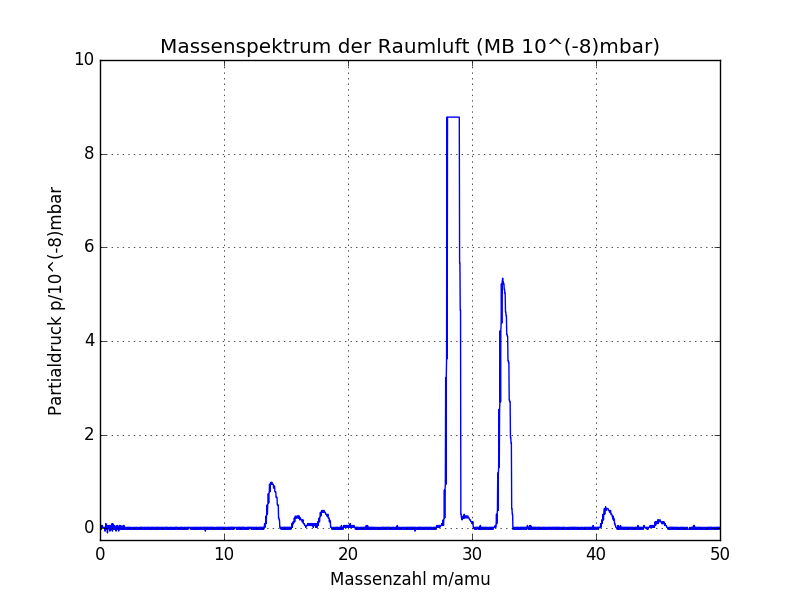
\includegraphics[width=0.9\textwidth]{fig/a4_2.png}
	\caption{Massenspektrum der Luft (Messbereich: $\SI{e-8}{\milli\bar}$)}
	\label{fig:v42}
\end{figure}

\begin{table}[tb]
 %\centering
 \caption{Massenspektrum der Luft}
 \label{tab:41}
 \hskip-1.0cm
 \begin{tabular}{ccccc} \toprule
   Massenzahl $/\si{\amu}$ & Bruchstück & Sensitivität $s$ & Peakhöhe $h/10^{-8}\si{\milli \bar}$ & Partialdruck $p/10^{-8}\si{\milli \bar}$ \\ \midrule
   $14$ & N$^{+}$ & $1,00$ & $0,94$ & $0,94$\\
   $16$ & O$^{+}$ & $0,62$ & $0,26$ & $0,42$ \\
   $18$ & H$_{2}$O$^{+}$ & $1,17$ & $0,38$ & $0,33$ \\
   $28$ & N$_{2}^{+}$ & $1,00$ & $27,3$ & $27,3$ \\
   $32$ & O$_{2}^{+}$ & $0,62$ & $5,42$ & $8,74$ \\
   $40$ & Ar$^{+}$ & $1,16$ & $0,46$ & $0,40$ \\
   $44$ & CO$_{2}^{+}$ & $0,9$ & $0,18$ & $0,20$ \\ \bottomrule
 \end{tabular}
\end{table}


\begin{table}[tb]
 \centering
 \caption{Messwerte für die Zusammensetzung der Luft}
 \label{tab:42}
 \begin{tabular}{ccc} \toprule
   Substanz & Anteil an der Raumluft $/\%$ & Literaturwert \cite{lubw} $/\%$ \\ \midrule
   Stickstoff & $73,69$ & $78,08$ \\
   Sauerstoff & $23,91$ & $20,95$ \\
   Wasserdampf & $0,85$ & - \\
   Argon & $1,04$ & $0,93$ \\
   Kohlendioxid & $0,52$ & $0,04$ \\ \bottomrule
 \end{tabular}

\end{table}


Die Partialdrücke sind in Tab. \ref{tab:41} aufgeführt. Für den Anteil eines Gases an der Raumluft gilt nun
\begin{equation}
 a = \frac{\sum_{i}p_{i}}{p_{\textrm{Ges}}},
\end{equation}
wobei $\sum_{i}p_{i}$ die Summe der Partialdrücke der Bruchstücke, in die ein Molekül zerfällt, bezeichnet. $p_{\textrm{Ges}}=\SI{38,32e-8}{\milli\bar}$ ist der Gesamtdruck der Komponenten. Es ist zu erkennen, dass $p_{\textrm{Ges}}$ deutlich geringer ist als der Gesamtdruck im Rezipienten.
Der Grund dafür ist vermutlich, dass nicht alle Gasmoleküle ionisiert werden.
Die Ergebnisse sind in Tab. \ref{tab:42} aufgeführt. Ein Vergleich mit Literaturwerten \cite{lubw} zeigt gute Übereinstimmung. Die Abweichung für Stickstoff beträgt ca. $6\%$, für Sauerstoff ca. $14\%$ und für Argon ca. $12\%$. Für Kohlendioxid beträgt die Abweichung jedoch ca. $1200\%$. Der Grund für die Abweichungen sind vermutlich Verunreinigungen im Rezipienten.
Möglicherweise wird die Messung auch dadurch beeinflusst, dass sich im Versuchsraum den ganzen Nachmittag über mehrere Personen aufhielten. Dies könnte zu einer Erhöhung des Kohlendioxidgehalts führen.

\subsection{Abhängigkeit des Partialdrucks vom Emissionsstrom}

In diesem Versuch wurde außerdem noch (in Absprache mit dem Betreuer, anstelle bei Versuchsteil $1$) die Abhängigkeit des Partialdrucks vom Emissionsstrom der Elektronenquelle gemessen. Dazu wurde die Linie $m=\SI{28}{\amu}$ verwendet, da diese am stärksten auftritt.
Es ergibt sich wie erwartet, dass der Partialdruck mit steigendem Emissionsstrom steigt (s. Abb. \ref{fig:v43}). Um also ein möglichst deutliches Ergebnis zu erhalten, ist es also sinnvoll den Emissionsstrom möglichst hoch einzustellen. Dies rechtfertigt, dass der Emissionsstrom bei allen Versuchsteilen auf $\SI{1}{\milli\ampere}$ eingestellt wird.

\begin{figure}[tb]
	\centering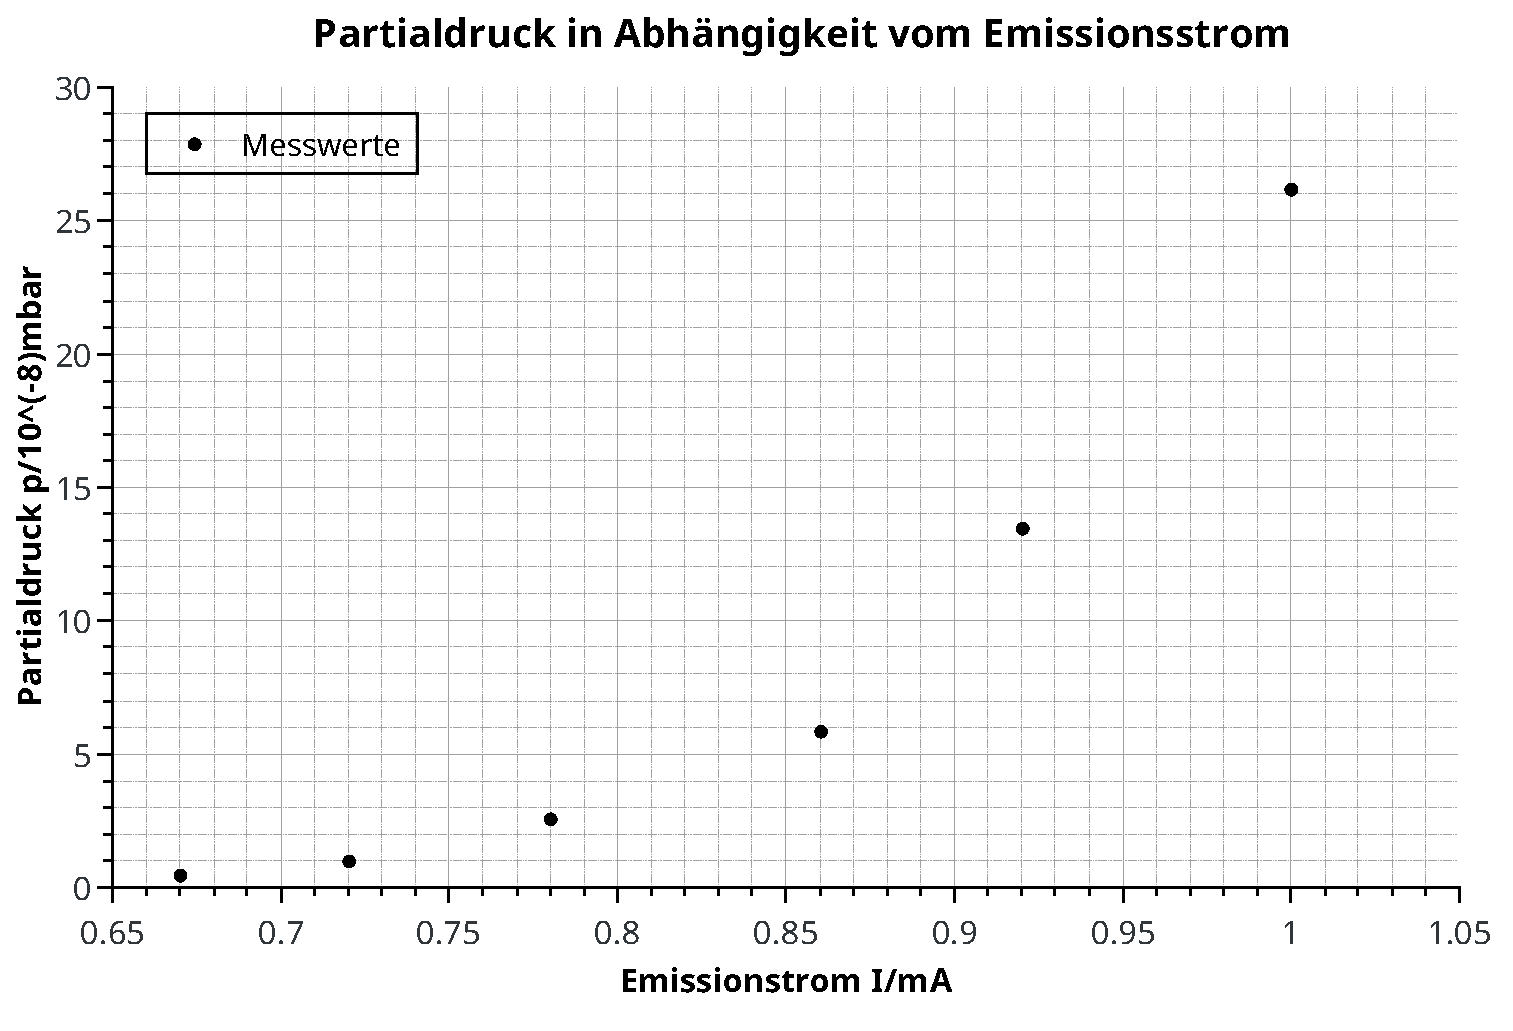
\includegraphics[width=0.8\textwidth]{fig/a4_emissionsstrom.pdf}
	\caption{Messwerte für den Partialdruck in Abhängigkeit des Emissionsstroms}
	\label{fig:v43}
\end{figure}

\section{Versuch 5: Qualitative Analyse}

In diesem Versuch wird das Massenspektrum eines unbekannten Gases bei den Energien $15, \, 30$ und $\SI{60}{\electronvolt}$ aufgenommen. Wie erwartet zeigen die Spektren bei $30$ und $\SI{60}{\electronvolt}$ (s. Abb. \ref{fig:v52} und \ref{fig:v53}) deutlich mehr Linien, als das Spektrum bei $\SI{15}{\electronvolt}$ (s. Abb. \ref{fig:v51}).
In diesem sind nur die Linien bei $28, \, 29, \, 44$ und $\SI{45}{\amu}$ deutlich zu erkennen. Im folgenden wird zur Ermittlung des unbekannten Gases das Spektrum bei $\SI{60}{\electronvolt}$ verwendet (s. Tab. \ref{tab:v5}).

Am deutlichsten im Spektrum zu sehen sind zum Einen die vier Linien bei $26, \, 27, \, 28$ und $\SI{29}{\amu}$. Die Linie $29$ gehört dabei zum Bruchstück $\textrm{C}_{2}\textrm{H}_{5}$ (und die anderen Linien entsprechend zu $\textrm{C}_{2}\textrm{H}_{4}$, etc.).
Diese Bruchstücke sind in allen Kohlenwasserstoffen zu sehen, da sie besonders stabil sind. Des Weiteren sind die Linien bei $39$ bis $\SI{45}{\amu}$ auffällig. Die Linie bei $44$ deutet darauf hin, dass es sich bei dem untersuchten Gas um Propan ($\textrm{C}_{3}\textrm{H}_{8}$) handelt.
Ein genauerer Vergleich mit dem Massenspektrum von Propan (s. Abb. \ref{fig:v54}) zeigt eine gute Übereinstimmung. Lediglich die Linie bei $45$ fällt etwas aus der Reihe, da deren Intensität deutlich höher ist, als erwartet.
Möglicherweise sind der Grund dafür Verunreinigungen, oder es kam bei Kollisionen der Moleküle zur Bildung von $\textrm{C}_{3}\textrm{H}_{9}^{+}$.

\begin{table}[tb]
 \centering
 \caption{Massenspektrum des unbekannten Gases bei $E=\SI{60}{\electronvolt}$}
 \label{tab:v5}
 \begin{tabular}{cccc} \toprule
   Massenzahl $/\si{\amu}$ & Bruchstück & Partialdruck $p/10^{-8}\si{\milli \bar}$ & relative Höhe \\ \midrule
   $15$ & CH$_{3}$ & $0,28$ & $0,03$\\
   $26$ & C$_{2}$H$_{2}$ & $0,52$ & $0,06$ \\
   $27$ & C$_{2}$H$_{3}$ & $2,80$ & $0,35$ \\
   $28$ & C$_{2}$H$_{4}$ & $5,12$ & $0,63$ \\
   $29$ & C$_{2}$H$_{5}$ & $8,12$ & $1,00$ \\
   $37$ & C$_{3}$H & $0,20$ & $0,02$ \\
   $38$ & C$_{3}$H$_{2}$ & $0,36$ & $0,04$ \\
   $39$ & C$_{3}$H$_{3}$ & $1,28$ & $0,16$ \\
   $41$ & C$_{3}$H$_{5}$ & $1,20$ & $0,15$ \\
   $44$ & C$_{3}$H$_{8}$ & $2,32$ & $0,29$ \\
   $45$ & & $2,56$ & $0,32$ \\ \bottomrule
 \end{tabular}
\end{table}


\begin{figure}[tb]
	\centering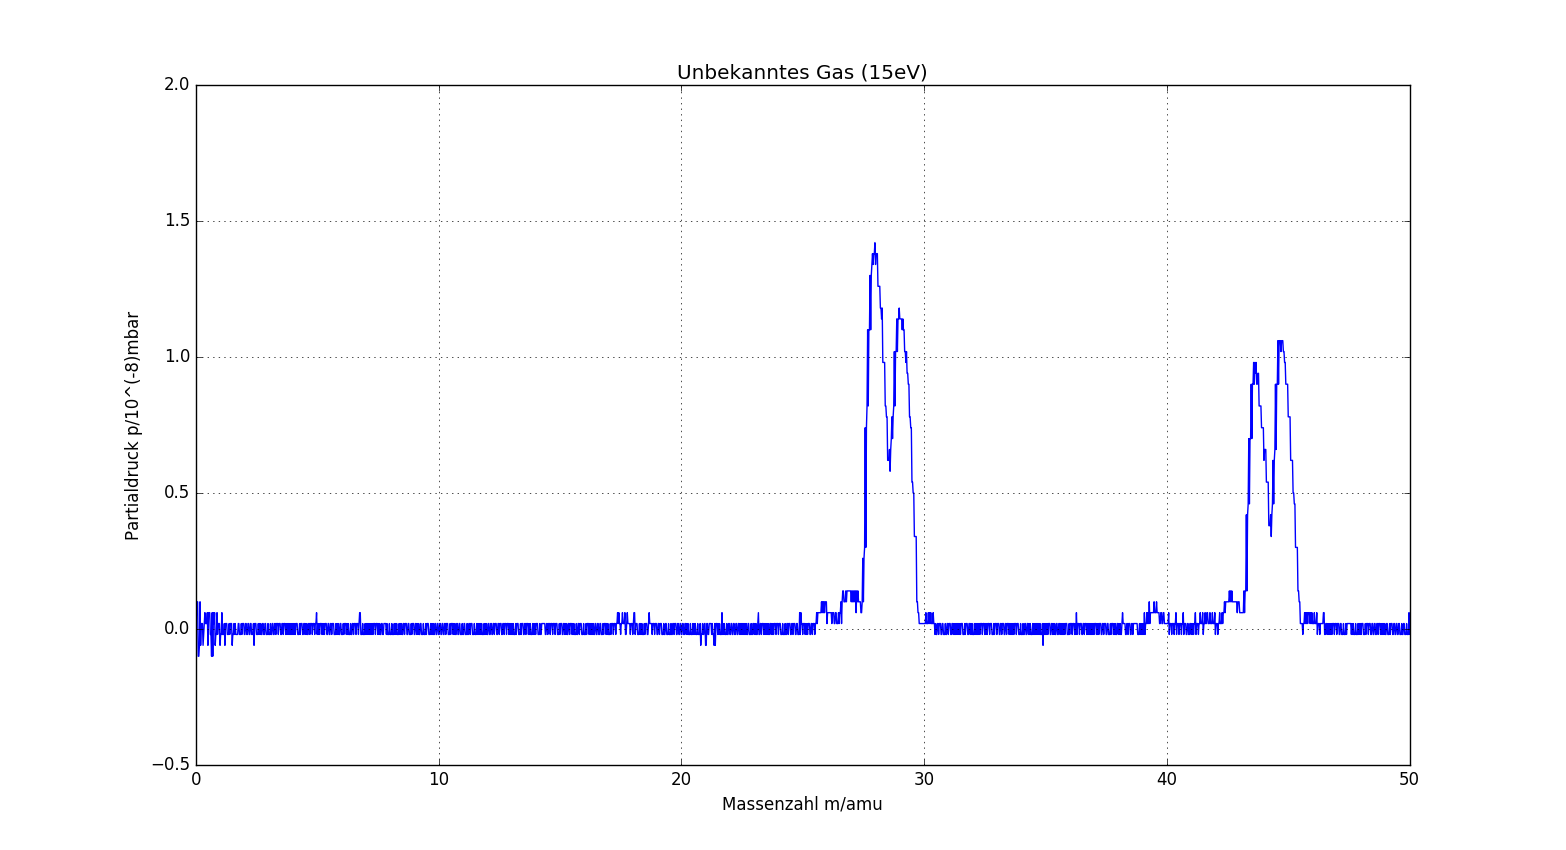
\includegraphics[width=1.1\textwidth]{fig/a5_15ev.png}
	\caption{Gemessenes Spektrum bei $E=\SI{15}{\electronvolt}$}
	\label{fig:v51}
\end{figure}

\begin{figure}[tb]
	\centering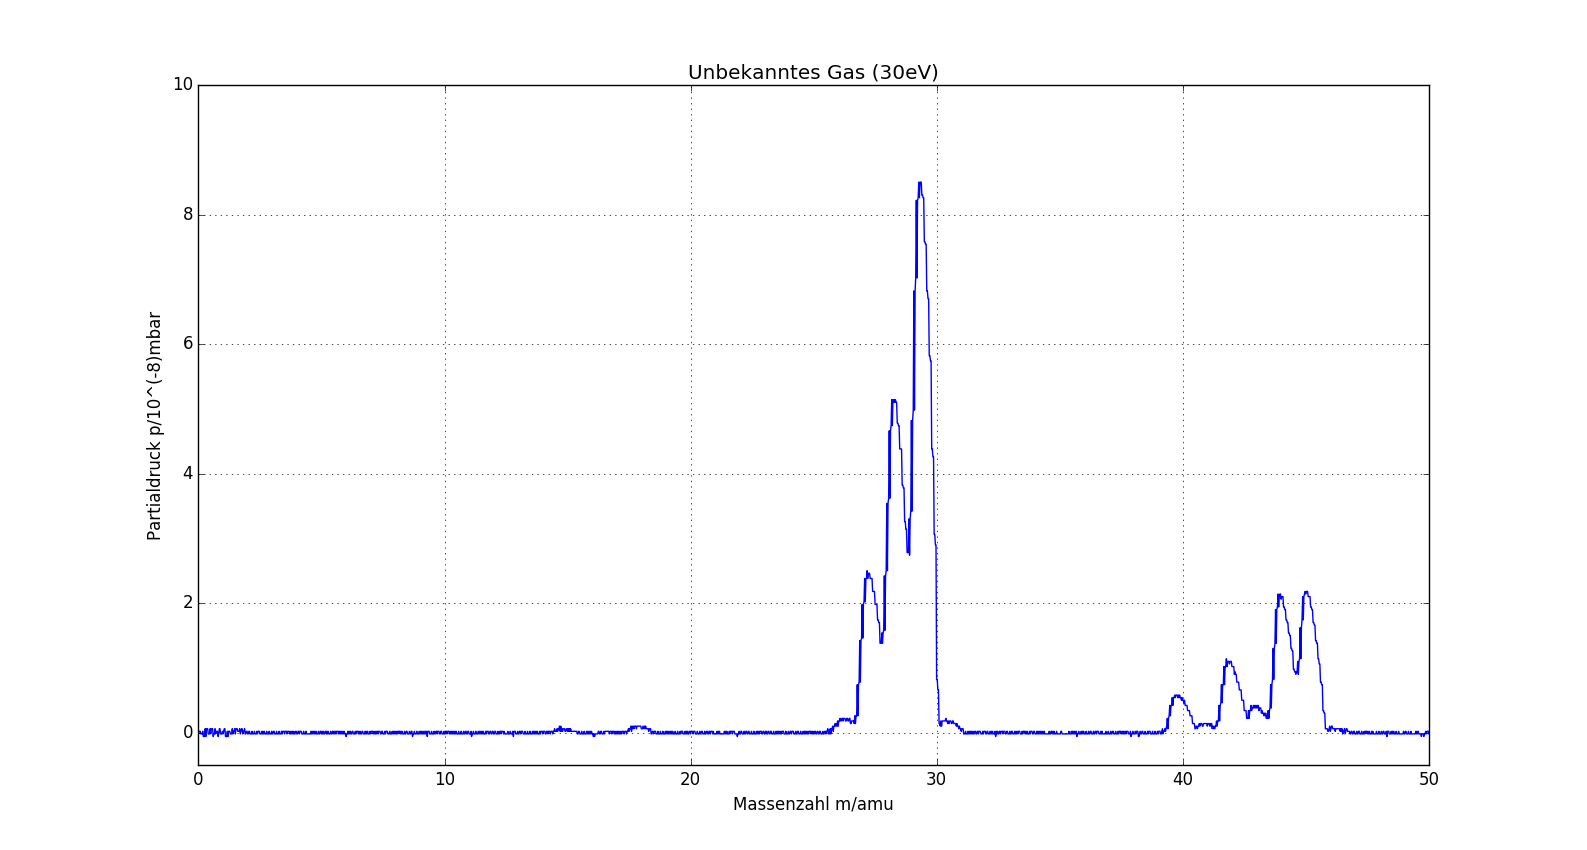
\includegraphics[width=1.1\textwidth]{fig/a5_30ev.png}
	\caption{Gemessenes Spektrum bei $E=\SI{30}{\electronvolt}$}
	\label{fig:v52}
\end{figure}

\begin{figure}[tb]
	\centering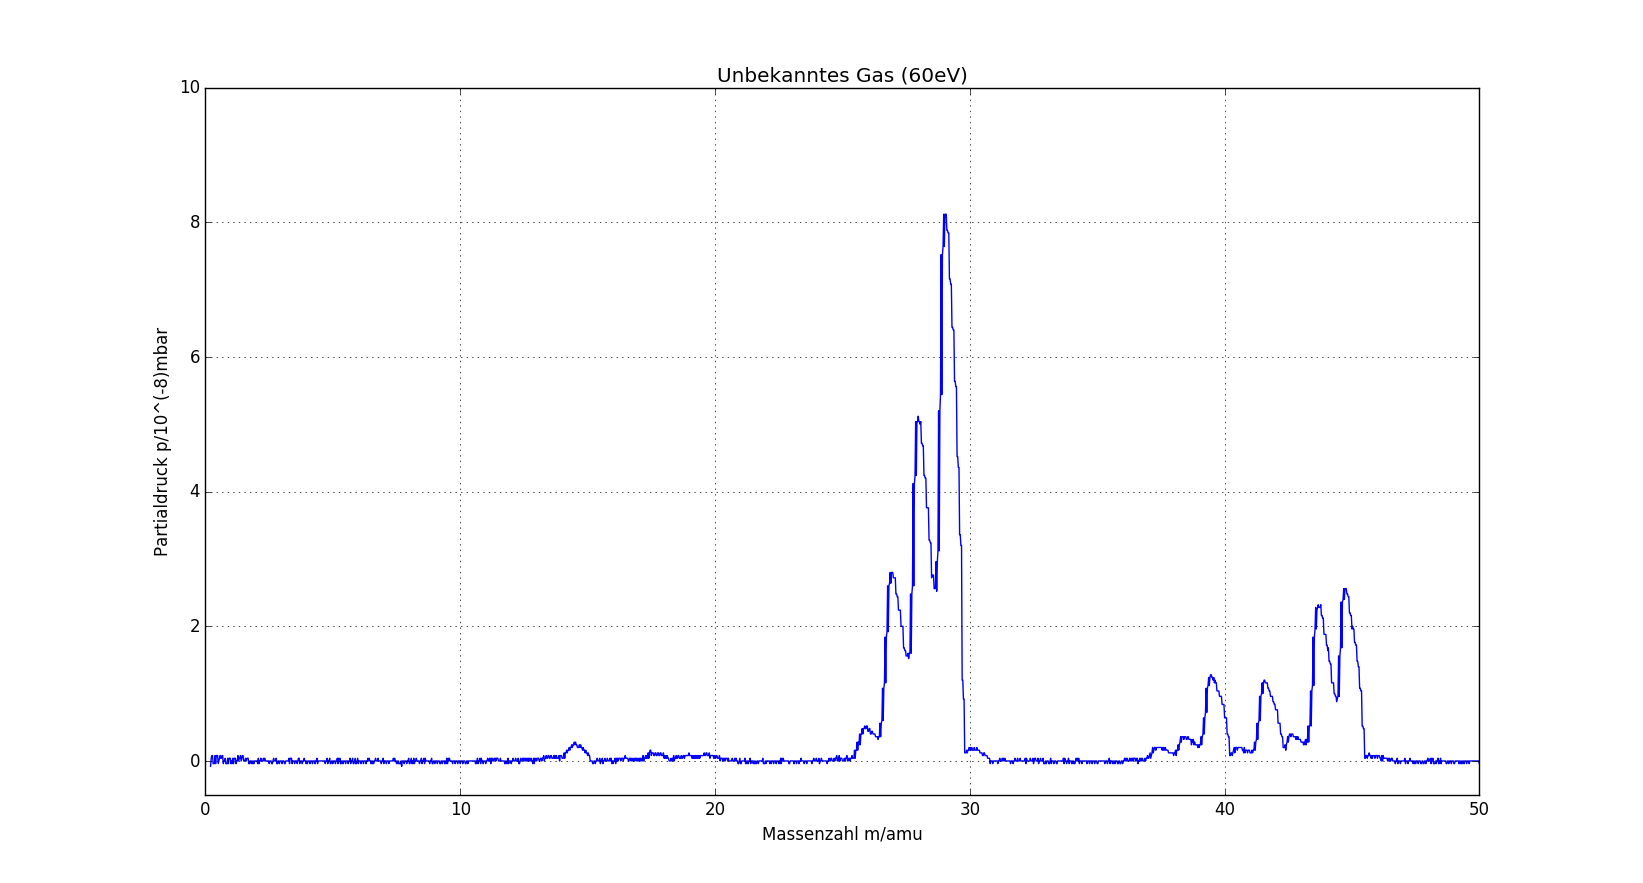
\includegraphics[width=1.1\textwidth]{fig/a5_60ev.png}
	\caption{Gemessenes Spektrum bei $E=\SI{60}{\electronvolt}$}
	\label{fig:v53}
\end{figure}

\begin{figure}[tb]
	\centering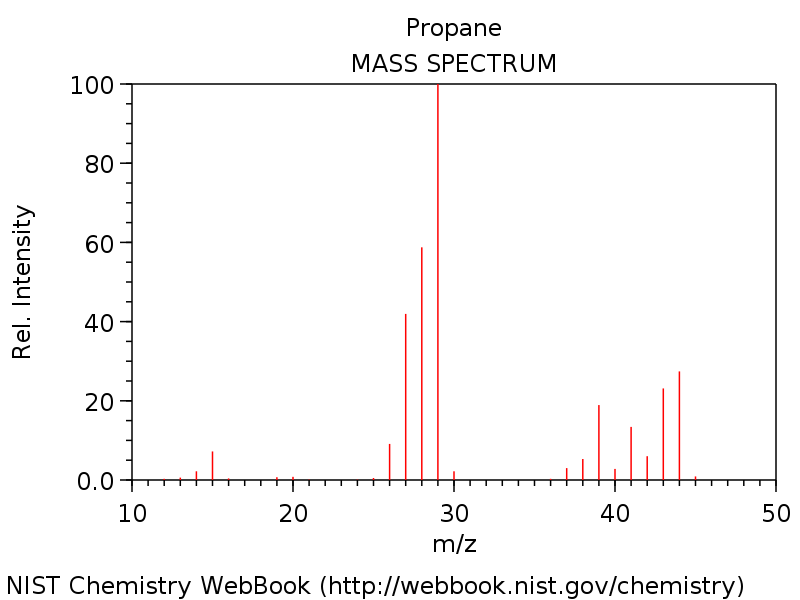
\includegraphics[width=0.9\textwidth]{fig/propan.png}
	\caption{Massenspektrum von Propan (Quelle: \cite{Nist})}
	\label{fig:v54}
\end{figure}

\section{Versuch 6: Zersetzungsenthalpie}

In diesem Versuch wird die Zersetzungsenthalpie $\Delta H$ von kohlesaurem Kalk (CaCO$_{3}$) zu CO$_{2}$ mit Hilfe der Massenspektrometrie bestimmt.
Erhitzt man kohlesauren Kalk, so bildet sich gasförmiges Kohlenstoffdioxid. Mit dem Massenspektrometer kann der Partialdruck des CO$_{2}$ gemessen werden. Da die Turbomolekularpumpe den Inhalt des Rezipienten fortlaufend abpumpt, kann die Reaktionsrate $k$ bis auf einen konstanten Faktor mit dem Partialdruck identifiziert werden.
Für die Reaktionsrate gilt die Arrhenius-Gleichung (\cite{wiki})
\begin{equation}
 k = A \exp\left(-\frac{\Delta H}{RT} \right),
\end{equation}
mit der Temperatur $T$, der allgemeinen Gaskonstante $R$ und einer reaktionsspezifischen Konstante $A$. Diese Gleichung lässt sich schreiben als
\begin{equation}
 \ln\left(\frac{p}{p_{0}}\right) = -\frac{\Delta H}{RT} + C,
\end{equation}
mit Konstanten $p_{0}$ und $C$. Wird der Partialdruck in Abhängigkeit von der Temperatur gemessen, so kann aus der Steigung $\Delta H$ bestimmt werden.

Im Versuch wurde die Temperatur mit einem Thermoelement gemessen. Dessen Spannungsanzeige lässt sich mit dem folgenden Zusamenhang in eine Temperatur umrechnen:
\begin{equation}
 T(V) = \SI{17,8571}{\kelvin\per\milli\volt} \cdot V + \SI{274,286}{\kelvin}.
\end{equation}
Für die lineare Regression wurden nur die Messwerte (s. Abb. \ref{fig:v61} ) mit $T\geq\SI{575}{\kelvin}$ verwendet, da die Zersetzungsrate für kleine Temperaturen zu gering ist. Die lineare Regression (\ref{fig:v62}) der Form $\ln\left(\frac{p}{p_{0}}\right)\left(\frac{1}{T}\right) = \frac{a}{T} + b$ wird mit ``Qtiplot'' durchgeführt und ergibt
\begin{align}
 a &= -\SI{14150\pm150}{\kelvin}, \\
 b &= 24,4 \pm 0,2,
\end{align}
wobei $p_{0}=\SI{e-8}{\milli\bar}$ gewählt wurde. Somit ergibt sich
\begin{equation}
 \Delta H = -Ra = \SI{117}{\kilo\joule\per\mol},
\end{equation}
mit einer statistischen Unsicherheit von
\begin{equation}
 \sigma_{\Delta H} = \SI{1}{\kilo\joule\per\mol}.
\end{equation}

Die systematische Unsicherheit ergibt sich folgendermaßen: Aus der systematischen Unsicherheit auf die Spannung des Thermoelements $\Delta V=\SI{0,05}{\milli\volt}$ (abgeschätzt) ergibt sich per Fehlerfortpflanzung
\begin{equation}
 \Delta T = \left| \frac{\partial T}{\partial V}\right| = \SI{17,8571}{\kelvin\per\milli\volt} \Delta V = \SI{0,89}{\kelvin}.
\end{equation}
Des Weiteren ist die Unsicherheit $\Delta p=\SI{1e-9}{\milli\bar}$ (abgeschätzt) zu berücksichtigen. Da die Unsicherheiten unkorreliert sind, ergibt sich per Gaußscher Fehlerfortpflanzung
\begin{equation}
 \Delta_{\textrm{syst}} = R \sqrt{\left(\ln\left(\frac{p}{p_{0}}\right)-b\right)^{2}\left(\Delta T\right)^{2} + \left(T\frac{\Delta p}{p}\right)^{2}} = \SI{0,2}{\kilo\joule\per\mol}
\end{equation}
Also ergibt sich insgesamt
\begin{equation}
 \Delta H = (117,6\pm1,2\pm0,2)\si{\kilo\joule\per\mole},
\end{equation}
wobei exemplarisch die Werte $T=\SI{625}{\kelvin}$ und $p=\SI{4e-8}{\milli\bar}$ verwendet wurden.
Der Literaturwert beträgt (bei $T=\SI{298}{\kelvin}$) \cite{chem}
\begin{equation}
 \Delta H = \SI{178,4}{\kilo\joule\per\mole}.
\end{equation}
Die Abweichung vom Literaturwert beträgt also ca. $34\%$ und liegt außerhalb der berechneten Fehlergrenzen. Der Literaturwert ist jedoch für $T=\SI{298}{\kelvin}$ gültig, und das Experiment wurde bei deutlich höherer Temperatur durchgeführt, was die Abweichung erklären könnte.



\begin{figure}[tb]
	\centering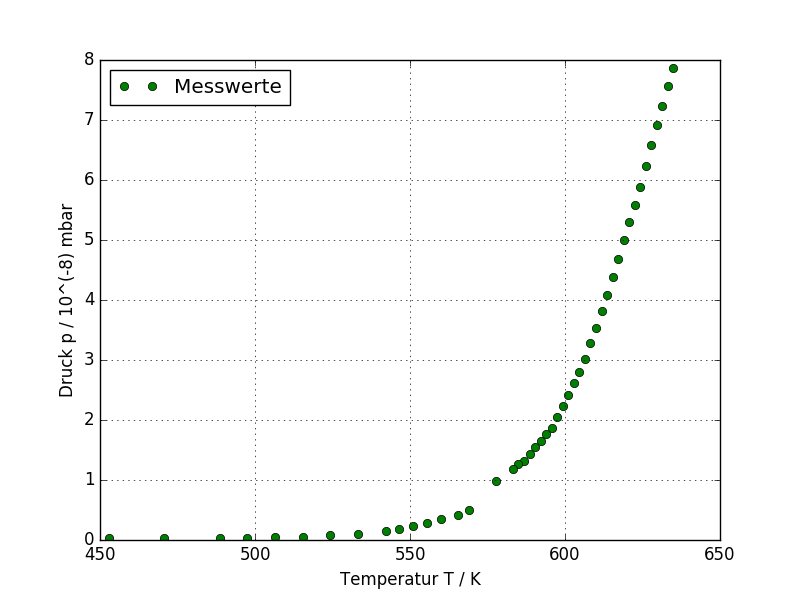
\includegraphics[width=0.9\textwidth]{fig/massen_a6_1.png}
	\caption{Messwerte für den Partialdruck $p$ in Abhängigkeit von der Temperatur $T$}
	\label{fig:v61}
\end{figure}

\begin{figure}[tb]
	\centering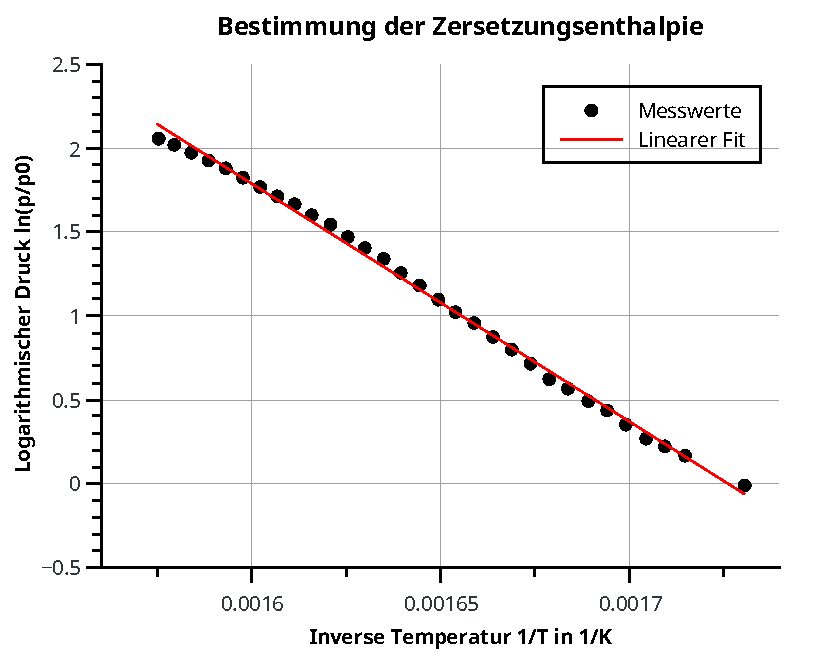
\includegraphics[width=0.9\textwidth]{fig/massen_a6_reg.pdf}
	\caption{Lineare Regression von $\ln\left(\frac{p}{p_{0}}\right)$ nach $\frac{1}{T}$}
	\label{fig:v62}
\end{figure}


%\begin{figure}[h]
%	\centering\includegraphics[width=0.8\textwidth]{fig/figure_4}
%	\caption{Extrem coole Grafik!}
%\end{figure}


% SUBFIGURE
%\begin{figure}[h]
%	\centering
%	\subfigure[]{\includegraphics[width=0.49\textwidth]{fig/2_a_plot}}
%	\subfigure[]{\includegraphics[width=0.49\textwidth]{fig/2_b_plot}}
%	\caption{\textbf{a)} Temperatur des Aluminium Hohlzylinders gegen die Zeit aufgetragen, \textbf{b)} Änderung der Temperatur gegenüber der Temperatur aufgetragen. Jeweils unter Verwendung des Heizdrahtes.}
%	\label{fig:2_1_plot}
%\end{figure}


